\section{Results}
\label{sec:results}

The results follow the order of the predictions. Money is in CLP billion. A $\pm$ interval is a standard deviation over
independent seeds unless a caption says otherwise. Table~\ref{tab:hypotheses}, at the end of the section, lists every prediction
with its measured value and whether it held.

\subsection{Structure of the committed aggregates}
\label{sec:results-structure}

All $\bdAggregates$ committed aggregates satisfy the structure of the rule (H1). Each has eight rows in the order of
Table~\ref{tab:protocol}, one row labelled headline capital and it is the simple sum, seven rows labelled information, one horizon
of one year and one level of 0.999, an Euler allocation and model-risk measures labelled information, and an Euler allocation
whose sum differs from the aggregate expected shortfall by a relative $\bdEulerGap$. The six aggregates reduce to $\bdDistinct$
distinct ones: the five documents carry one aggregation block, and the market-credit stress is the other. The simple sum and the
square-root row, recomputed by the engine from the committed marginal capital and the committed matrix, equal the committed rows
to a relative $10^{-12}$.

The two bound rows converge. The four rearrangements behind them ran $\bdSweeps$ sweeps, the range of the lower bound is CLP
\bdLowerRangeLo{} to \bdLowerRangeHi{} billion of value at risk, a width of \bdLowerRangeWidth{} billion, and the range of the
worst case is CLP \bdUpperRangeLo{} to \bdUpperRangeHi{} billion, a width of \bdUpperRangeWidth{} million. The worst value at risk
of CLP \bdWorstVar{} billion is below the ceiling of Proposition~\ref{prop:headline}, the sum of the expected shortfalls of the
marginals, CLP \bdSumEs{} billion, by CLP \bdSlack{} billion, and the comonotonic value at risk is CLP \bdComoVar{} billion: the
worst case is $\bdWorstOverEs$ of the ceiling and exceeds the comonotonic value, as the proposition allows. On the committed
aggregate the nine tests return green for seven and amber for two: the copula-choice statistic is $\bdCopulaStat$ percent, between
the green limit of 5 and the red limit of 15, and the correlation-stress statistic is $\bdStressStat$ percent, above the amber limit
of 10. The reference of Rosenberg and Schuermann reports an additive overestimate of $\bdRsOver$ percent for the case, inside their
published range of 30 to 40 percent.

\subsection{The band of Banco Andino}
\label{sec:results-band}

Table~\ref{tab:main-results} and Figure~\ref{fig:band} give the band. The headline is CLP \bdHeadline{} billion. The lower bound is
CLP \bdLower{} billion, a diversification factor of \bdLowerDf, and the worst case is CLP \bdWorst{} billion, a factor of \bdWorstDf{},
so the worst case lies $\bdWorstAbove$ percent above the headline. The band is CLP \bdWidth{} billion wide, $\bdWidthOverHeadline$ times
the headline. The interior rows fall between CLP \bdGauss{} billion for the Gaussian copula and CLP \bdTFour{} billion for the $t$
copula with 4 degrees of freedom; the Gaussian row is $\bdGaussBelow$ percent below the headline, which is the same fact as the
simple sum exceeding it by $\bdAdditiveOver$ percent.

\begin{table}[htbp]
\centering
\small
\caption{The dependence band of Banco Andino at one year and 99.9 percent in CLP billion: the committed rows with their Monte Carlo standard error and diversification factor against the simple sum, then the rows rebuilt by the engine from the committed marginal grids as mean and standard deviation over independent seeds (20 for the base matrix, 10 for the matrix with market-credit correlation 0.8) and the relative change under the stress. The two bound rows do not move with the matrix.}
\label{tab:main-results}
\fitwidth{\begin{tabular}{lrrrrr}
\toprule
Row & Committed & DF & Rebuilt, base & Rebuilt, market-credit 0.8 & Change \\
\midrule
\relax lower bound & \relax 118.5 & \relax 0.180 & \relax 118.5 $\pm$ 0.0 & \relax 118.5 $\pm$ 0.0 & \relax +0.000 \\
\relax simple sum (headline) & \relax 658.0 & \relax 1.000 & \relax 658.0 $\pm$ 0.0 & \relax 658.0 $\pm$ 0.0 & \relax +0.000 \\
\relax square-root rule & \relax 528.1 & \relax 0.803 & \relax 528.1 $\pm$ 0.0 & \relax 568.5 $\pm$ 0.0 & \relax +0.077 \\
\relax Gaussian copula & \relax 492.0 $\pm$ 2.5 & \relax 0.748 & \relax 488.1 $\pm$ 3.2 & \relax 549.7 $\pm$ 2.5 & \relax +0.126 \\
$t$ copula, $\nu=4$ & \relax 552.4 $\pm$ 3.4 & \relax 0.839 & \relax 546.9 $\pm$ 4.1 & \relax 584.4 $\pm$ 3.0 & \relax +0.068 \\
$t$ copula, $\nu=8$ & \relax 528.3 $\pm$ 2.8 & \relax 0.803 & \relax 522.7 $\pm$ 3.7 & \relax 572.4 $\pm$ 3.3 & \relax +0.095 \\
$t$ copula, $\nu=30$ & \relax 499.1 $\pm$ 3.3 & \relax 0.759 & \relax 498.8 $\pm$ 3.1 & \relax 558.3 $\pm$ 4.5 & \relax +0.119 \\
\relax worst case & \relax 823.3 & \relax 1.251 & \relax 823.3 $\pm$ 0.0 & \relax 823.3 $\pm$ 0.0 & \relax 0.000 \\
\bottomrule
\end{tabular}}
\end{table}


\begin{figure}[htbp]
\centering
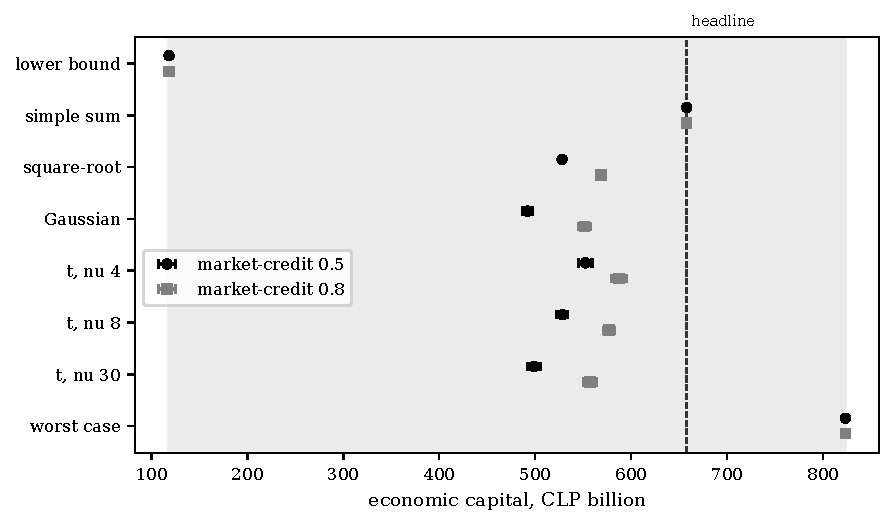
\includegraphics[width=0.86\textwidth]{figures/band}
\caption{The band of Banco Andino at one year and 99.9 percent: the capital of each row in CLP billion for the base matrix (circles) and for the matrix with market-credit correlation 0.8 (squares), with two standard errors where the row is simulated, the interval from the lower bound to the worst case shaded and the headline marked by the dashed line.}
\label{fig:band}
\end{figure}

\emph{Reproduction (H2).} The engine, run on the marginals rebuilt from the committed quantile grids with the committed seed,
returns every committed row to within \bdMaxRelDiff{} percent: the closed-form rows exactly, the lower bound to \bdLowerRelDiff{}
percent and the worst case to \bdWorstRelDiff{} percent (the random start of the rearrangement), and the Gaussian row to
\bdGaussRelDiff{} percent. Each difference is below the tolerance of three combined standard errors or half a percent. The
committed documents are therefore reproduced from the committed marginal grids alone, which is the property that lets a reader
check the band without the simulated samples. The $\bdRepsBase$ independent runs of Table~\ref{tab:main-results} show the sampling
variation: the standard deviation is CLP \bdGaussSd{} billion for the Gaussian row, CLP \bdTFourSd{} billion for the $t$ row with 4
degrees of freedom and at most CLP \bdMaxSd{} billion for any row, and $\bdBoundsSd$ billion for the bound rows.

\emph{The band is not noise (H3).} The width of CLP \bdWidth{} billion is \bdWidthOverSe{} times the largest Monte Carlo standard
error, CLP \bdMaxSe{} billion, which is above the 100 that the prediction required. No row speaks for the band: the largest relative difference from a row to another row is
$\bdFarthestMin$ percent for the Gaussian copula, the row with the smallest such difference, and rises to $\bdFarthestMax$ percent
for the lower bound. No single row is within three quarters of every other.

\emph{Invariance of the bounds (H5).} The stress that raises the market-credit correlation to 0.8 leaves the lower bound and the
worst case unchanged to the precision of the documents, as Proposition~\ref{prop:bracket} requires, while the Gaussian row moves by
$\bdGaussMove$ percent in the committed documents (the rebuilt means in Table~\ref{tab:main-results} show $+0.126$): above the 10
percent of the prediction. The $t$ rows move less, by $\bdTFourMove$ percent for 4 degrees of freedom, $\bdTEightMove$ percent
for 8 and $\bdTThirtyMove$ percent for 30, and the square-root row by $\bdVcMove$ percent. The ordering is that of the tail
dependence: the stress adds least where the $t$ copula already has the most tail dependence, and most where the copula has
almost none. After the stress the interior rows, CLP \bdGaussStress{} to \bdTFourStress{} billion, are still below the headline.

\subsection{The \texorpdfstring{$t$}{t} row as a function of the degrees of freedom}
\label{sec:results-nu}

Figure~\ref{fig:nu-curve} gives the capital of the $t$ copula row for eight values of $\nu$ and the two matrices. On the base
matrix it falls from CLP \bdTTwoFive{} billion at $\nu=2.5$ and \bdTThree{} at $\nu=3$ to \bdTHundred{} at $\nu=100$, a span of
CLP \bdNuSpanBase{} billion or $\bdNuSpanPc$ percent of the smallest value, and the curve approaches the Gaussian row, CLP \bdGauss{}
billion at the committed seed. The three values of the set, 4, 8 and 30, give CLP \bdTFour{}, \bdTEight{} and \bdTThirty{} billion at the committed seed, the last
within $\bdCopulaDiffThirty$ percent of the Gaussian row, so the set spans the curve from the heavy tail to the nearly Gaussian one;
the values below 4 are outside the set and lie within the noise of the value at 3.
The curve is monotone within two combined standard errors on both matrices, the evidence for the conjecture of
Section~\ref{sec:theory-tails}, and the segment from $\nu=2.5$ to $3$ is flat within the noise. The tail dependence coefficient at the pair
correlation of 0.5 falls over the same range from $\bdTLambdaTwoFive$ at $\nu=2.5$ to $\bdTLambdaThirty$ at $\nu=30$.

\begin{figure}[htbp]
\centering
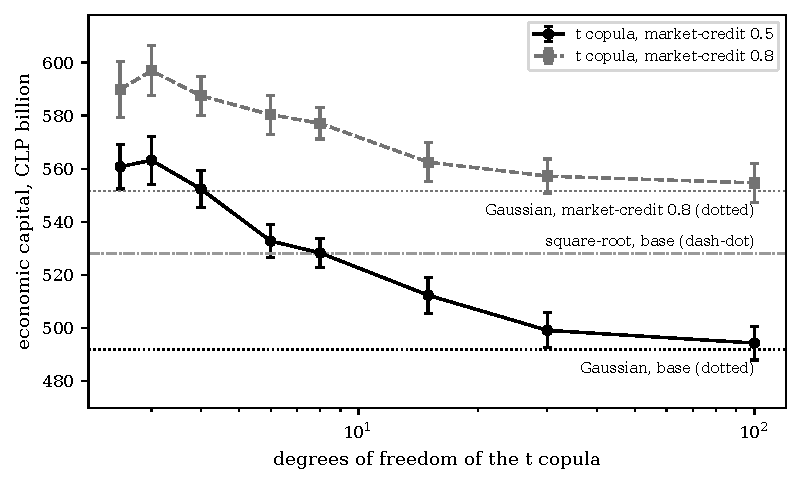
\includegraphics[width=0.82\textwidth]{figures/nu-curve}
\caption{The capital of the $t$ copula row against the degrees of freedom of the copula, in CLP billion, for the base matrix (solid) and for the matrix with market-credit correlation 0.8 (dashed), with two standard errors of each estimate from one run of $10^6$ draws. The dotted lines are the Gaussian copula row of each matrix and the dash-dotted line the square-root row of the base matrix.}
\label{fig:nu-curve}
\end{figure}

\subsection{Planted dependence structures}
\label{sec:results-planted}

Table~\ref{tab:planted-truth} and Figure~\ref{fig:truth-errors} set the rows of the band against the ten planted structures. The
capital of a structure ranges from CLP \bdTruthMin{} billion for independent risks to CLP \bdTruthMax{} billion for the $t$ copula with 3
degrees of freedom and the crisis matrix, which is $\bdTruthMaxOverHeadline$ of the headline and $\bdTruthMaxOverWorst$ of the worst case. The
standard error of every capital is at most CLP \bdTruthSeMax{} billion.

\begin{table*}[htbp]
\centering
\small
\caption{Ten planted dependence structures on the marginals of Banco Andino: the capital of the structure in CLP billion with its standard error over independent samples, the relative error in percent of the Gaussian copula row, of the square-root row, of the hybrid quantile with the correlation of the structure and of the Gaussian copula with its rank correlation, and whether the interior rows (hull), the interior rows of both matrices (hull+s) and the sharp range from the lower bound to the worst case contain it.}
\label{tab:planted-truth}
\fitwidth{\begin{tabular}{lrrrrrccc}
\toprule
Planted structure & Capital & Gauss. & Sqrt & Hybrid & Gauss. rank & Hull & Hull+s & Range \\
\midrule
\relax Gaussian, base matrix & \relax 487.9 $\pm$ 0.65 & \relax +0.0 & \relax +8.2 & \relax +0.9 & \relax -0.7 & \relax yes & \relax yes & \relax yes \\
\relax Gaussian, market-credit 0.8 & \relax 551.1 $\pm$ 1.06 & \relax -11.4 & \relax -4.2 & \relax -3.7 & \relax -0.6 & \relax no & \relax yes & \relax yes \\
\relax Gaussian, crisis matrix & \relax 575.9 $\pm$ 0.67 & \relax -15.3 & \relax -8.3 & \relax -4.1 & \relax +0.3 & \relax no & \relax yes & \relax yes \\
\relax Gaussian, independent risks & \relax 348.8 $\pm$ 0.45 & \relax +39.9 & \relax +51.4 & \relax +3.0 & \relax -0.3 & \relax no & \relax no & \relax yes \\
\relax t copula, 3 degrees, base matrix & \relax 555.6 $\pm$ 0.78 & \relax -12.2 & \relax -5.0 & \relax -8.9 & \relax -12.2 & \relax no & \relax yes & \relax yes \\
\relax t copula, 2.5 degrees, base matrix & \relax 560.9 $\pm$ 0.76 & \relax -13.0 & \relax -5.9 & \relax -12.2 & \relax -12.9 & \relax no & \relax yes & \relax yes \\
\relax t copula, 3 degrees, crisis matrix & \relax 611.1 $\pm$ 0.56 & \relax -20.1 & \relax -13.6 & \relax -9.1 & \relax -6.2 & \relax no & \relax no & \relax yes \\
\relax Gaussian regimes, 5 percent crisis & \relax 493.7 $\pm$ 0.57 & \relax -1.1 & \relax +7.0 & \relax +1.4 & \relax -0.9 & \relax yes & \relax yes & \relax yes \\
\relax Clayton, reflected, same mean tau & \relax 583.2 $\pm$ 1.10 & \relax -16.3 & \relax -9.4 & \relax -17.5 & \relax -21.8 & \relax no & \relax yes & \relax yes \\
\relax Gumbel, same mean tau & \relax 577.0 $\pm$ 1.13 & \relax -15.4 & \relax -8.5 & \relax -17.7 & \relax -21.7 & \relax no & \relax yes & \relax yes \\
\bottomrule
\end{tabular}}
\end{table*}


\begin{figure}[htbp]
\centering
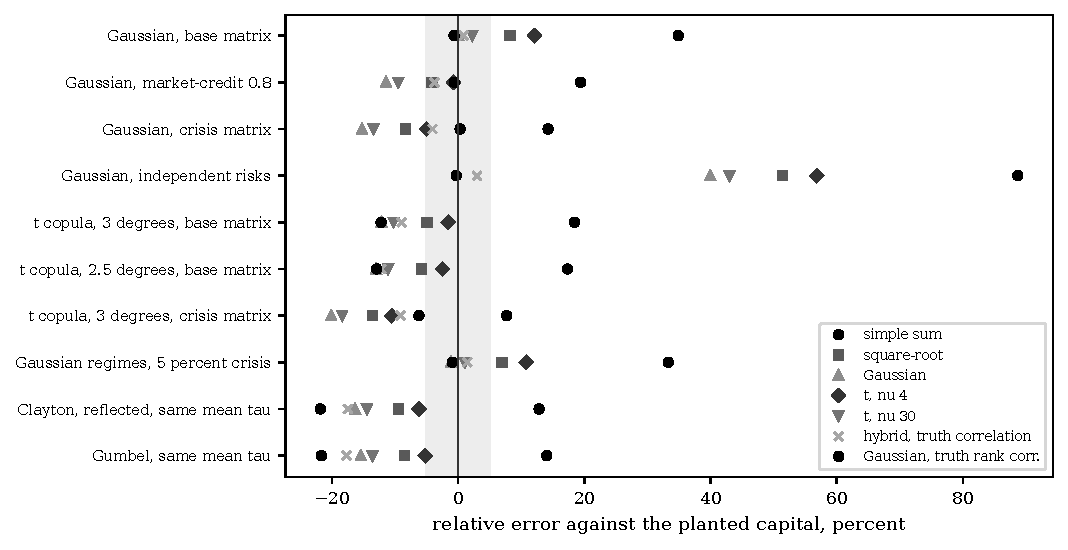
\includegraphics[width=0.92\textwidth]{figures/truth-errors}
\caption{Relative error in percent of six single-figure methods against the planted capital of each of the ten structures: the simple sum, the square-root row, the Gaussian copula row, the $t$ rows with 4 and 30 degrees of freedom, the hybrid quantile and the Gaussian copula calibrated on the structure itself. The shaded band marks errors within 5 percent; each marker is one method on one structure.}
\label{fig:truth-errors}
\end{figure}

\emph{Coverage by the sharp range (H4a).} The range from the lower bound to the worst case contains all $\bdCovSharp$ capitals,
which is Proposition~\ref{prop:coverage} met by the implementation. The range is wide: its median width is $\bdAblFullWidth$ times the
capital of the structure, and even the structure with the heaviest dependence is $\bdTruthMaxOverWorst$ of the worst case, so
the worst case is an outer bound and not a scenario.

\emph{Coverage by the interior rows (H4b, refuted).} The interval spanned by the five interior rows of the base matrix contains the
capital of $\bdCovInterior$ of the ten structures, the Gaussian copula with the base matrix, which is one of the rows, and the mixture
in which 95 percent of the draws follow it; the prediction required at least 75 percent. When the interior rows of the stressed
matrix are added, the interval contains $\bdCovInteriorStress$ of ten, and it misses independent risks, below the interval, and
the $t$ copula with 3 degrees of freedom and the crisis matrix, above it. The reflected Clayton copula is inside the interval, close to its upper end. The prediction on the interior rows alone is refuted; what the
interior rows cover depends on the matrix that is among them.

\emph{A single figure is not reliable (H4c).} The Gaussian row is within 5 percent of the capital in $\bdGaussWithin$ of the ten
structures, the structure that is Gaussian with the base matrix, where it is exact, and the mixture. Its absolute error has a median
of $\bdGaussMedErr$ percent and a maximum of $\bdGaussMaxErr$ percent, for independent risks, and it underestimates every structure that
has more dependence than the base matrix: with relative errors of $\bdGaussErrGaussianStress$ percent for the stressed matrix and
$\bdGaussErrTthreeCrisis$ percent for the heavy $t$ structure. The simple sum overestimates every structure and by up to
$\bdSumMaxErr$ percent. The prediction held.

The two estimators calibrated on the structure itself are better and not good. The hybrid quantile has a median absolute error of
$\bdHybridMedErr$ percent and a maximum of $\bdHybridMaxErr$ percent, and the Gaussian copula with the rank correlation of the
structure has a median of $\bdKendallMedErr$ percent and a maximum of $\bdKendallMaxErr$ percent. The latter is within $\bdKGaussMax$ percent for
all four Gaussian structures and for the mixture, because the Gaussian copula is the right family there, and it underestimates by $\bdKTailMin$
to $\bdKTailMax$ percent the $t$ and the two non-elliptical structures, whose tail dependence a matrix of rank correlations cannot carry
(Proposition~\ref{prop:tails}). A bank with a long history and a perfect estimate of the matrix would still need the band.

\subsection{The common horizon and level}
\label{sec:results-level}

Reading the market marginal at 99 percent in place of 99.9 percent lowers its capital from CLP \bdEcMarket{} to
CLP \bdMarketEcNineNine{} billion, a change of $\bdMarketEcChange$ percent, and lowers the simple sum to CLP \bdSumMismatch{}
billion, a change of $\bdHeadlineChange$ percent: a headline that looks like an aggregate at 99.9 percent and mixes two levels (H6).
The consistency test returns red on that band, and also on a band in which one marginal is read at a ten-day horizon, and green on
the consistent one. The engine itself refuses the band with the unconverted capital: the capital of the market marginal does not match
its quantile function at the level of the band within the tolerance of 1 percent. The two defences are independent, the test on the
metadata and the refusal on the values, and the prediction held. The size of the effect is that of the arithmetic of the
quantiles: the market marginal has no expected loss and carries $\bdEcShareMarket$ percent of the sum of the capital figures, so a
change of $\bdMarketEcChange$ percent in its capital moves the sum by about $\bdEcShareMarket$ percent of that, which is the
$\bdHeadlineChange$ percent observed. A change of this size in the headline is not a small inconsistency, and the aggregate that
results has no meaning as a quantile of any loss.

\subsection{Allocation and model-risk measures}
\label{sec:results-allocation}

Table~\ref{tab:euler} and Figure~\ref{fig:euler} give the Euler allocation of the expected shortfall of the Gaussian copula
aggregate over $20$ seeds. The aggregate expected shortfall is CLP \bdEsTotalMean{} $\pm$ \bdEsTotalSd{} billion, which contains the
committed value of CLP \bdEsTotal{} billion, and the contributions add up to it with a relative gap of at most $\bdEulerMaxGap$ in every
seed. The shares of the four risk types are $\bdShareCredit\pm\bdShareSdCredit$, $\bdShareMarket\pm\bdShareSdMarket$,
$\bdShareIrrbb\pm\bdShareSdIrrbb$ and $\bdShareOperational\pm\bdShareSdOperational$ percent. The allocation by stand-alone expected
shortfall sums to CLP \bdSumStandaloneEs{} billion, $\bdStandaloneOver$ times the aggregate, and over-allocates to the operational risk in
particular, whose benefit of diversification by the Euler allocation is $\bdBenefitOperational$ percent against $\bdBenefitCredit$,
$\bdBenefitMarket$ and $\bdBenefitIrrbb$ percent for credit, market and interest rate risk.

\begin{table}[htbp]
\centering
\small
\caption{The Euler allocation of the expected shortfall of the Gaussian copula aggregate at 99.9 percent in CLP billion, as mean over independent seeds with the standard deviation of the share, against the stand-alone expected shortfall of each marginal, which sums to more than the aggregate; the benefit is one minus the contribution over the stand-alone figure.}
\label{tab:euler}
\fitwidth{\begin{tabular}{lrrrrr}
\toprule
Risk & Euler contribution & Share, percent & Stand-alone ES & Share, percent & Benefit, percent \\
\midrule
\relax credit & \relax 258.5 & \relax 36.7 $\pm$ 1.2 & \relax 346.9 & \relax 35.4 & \relax 25 \\
\relax market & \relax 276.7 & \relax 39.3 $\pm$ 1.3 & \relax 355.8 & \relax 36.3 & \relax 22 \\
\relax IRRBB & \relax 78.5 & \relax 11.2 $\pm$ 0.3 & \relax 106.4 & \relax 10.9 & \relax 26 \\
\relax operational & \relax 90.0 & \relax 12.8 $\pm$ 2.7 & \relax 171.1 & \relax 17.5 & \relax 47 \\
\relax sum & \relax 703.7 & \relax 100.0 & \relax 980.2 & \relax 100.0 & \relax -- \\
\bottomrule
\end{tabular}}
\end{table}


\begin{figure}[htbp]
\centering
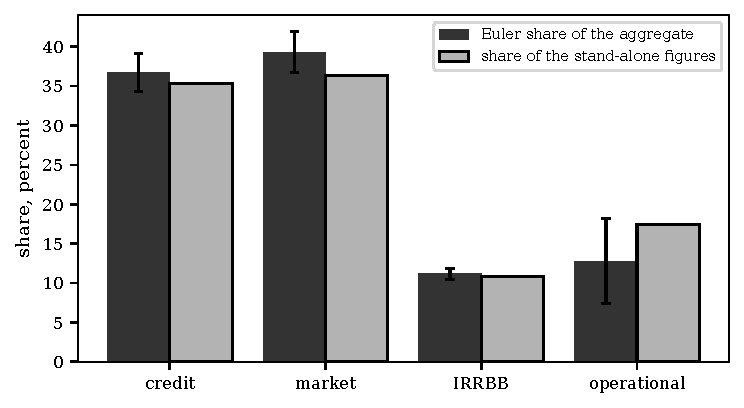
\includegraphics[width=0.7\textwidth]{figures/euler}
\caption{Share of each risk type in the aggregate expected shortfall of the Gaussian copula row at 99.9 percent: the Euler allocation (dark bars, mean over 20 seeds with two standard deviations) and the share in the sum of the stand-alone expected shortfalls (light bars), which does not describe the aggregate.}
\label{fig:euler}
\end{figure}

The model-risk measures of the band are information. With the Gaussian copula as the reference model, the additive measure is
$\bdAm$ percent and the relative measure is $\bdRm$: multiplying the Gaussian row by the factor $1+\mathrm{AM}$ reaches the worst
case, and the worst case lies above the Gaussian row by $\bdRmPct$ percent of the width of the band. The measure of Glasserman and Xu
with a relative entropy budget of $\bdGxEta$ raises the expected aggregate loss from CLP \bdGxBase{} to \bdGxWorst{} billion.

\subsection{The predictions}
\label{sec:results-hypotheses}

\begin{table}[htbp]
\centering
\small
\caption{The predictions stated before the experiments, the measured quantity of each and whether it held or was refuted, from the outputs of the experiment scripts.}
\label{tab:hypotheses}
\fitwidth{\begin{tabular}{llp{5.2cm}l}
\toprule
Id & Prediction & Measured & Outcome \\
\midrule
\relax H1 & \relax structure of the band in six committed aggregates & \relax 6 of 6 pass & \relax held \\
\relax H2 & \relax rebuilt rows reproduce the committed rows & \relax largest difference 0.0075 percent & \relax held \\
\relax H3 & \relax band wider than 100 standard errors; no row speaks for it & \relax width 205 s.e.; closest row 76 percent from another & \relax held \\
\relax H4a & \relax sharp range contains every planted capital & \relax 10 of 10 & \relax held \\
\relax H4b & \relax interior rows contain at least 75 percent of planted capitals & \relax 2 of 10 (8 with the stressed matrix) & \relax refuted \\
\relax H4c & \relax Gaussian row within 5 percent in at most half & \relax 2 of 10 & \relax held \\
\relax H5 & \relax bounds invariant to the matrix; Gaussian row moves over 10 percent & \relax bounds differ by 0; Gaussian row moves 12.1 percent & \relax held \\
\relax H6 & \relax level mismatch changes the sum over 10 percent and the test is red & \relax sum -17.9 percent; test red & \relax held \\
\relax H7 & \relax tests need the rows; Gaussian row alone runs at most half & \relax 6 of 9 run on the Gaussian row & \relax refuted \\
\bottomrule
\end{tabular}}
\end{table}


Table~\ref{tab:hypotheses} lists the outcome of each prediction. Seven of the nine held and two were refuted. The structure of the
rule (H1), the reproduction of the committed band (H2), the width of the band relative to its sampling error (H3), the coverage by
the sharp range (H4a), the weakness of a single Gaussian figure (H4c), the invariance of the bounds (H5) and the effect of an
unconverted level (H6) held. The coverage of the planted structures by the interior rows of the base matrix (H4b) was refuted,
with 2 of 10 against the 75 percent predicted, and the second clause of the prediction on the tests (H7) was refuted: six of the
nine tests, not at most half, can be run on the Gaussian row alone (Section~\ref{sec:ablation}). The two refuted predictions
concern the interior rows and the tests, not the structure of the rule or the reproduction of the band; Section~\ref{sec:discussion-failures}
discusses them. The measured column of the table keeps the units of the thresholds, so that a margin can be read: the width is
\bdWidthOverSe{} standard errors against 100, the Gaussian row moves $\bdGaussMove$ percent against 10, and the level mismatch moves the
sum by $\bdHeadlineChange$ percent against 10.
